\chapter{Límites y continuidad}

\newpage
\section{Definición de límite}

Es usual que al comienzo de un curso de cálculo o pre-cálculo, se estudie el concepto de límite y por tanto, su definición formal. El límite es un concepto de suma importancia en la matemática, pues permitió formalizar el cálculo de áreas, volúmenes y razones de cambio instantáneas.

\noindent
\begin{minipage}[t]{0.6\textwidth}
\hspace*{0.65cm}La demostración más famosa, mediante \textit{épsilon-delta} ($\varepsilon-\delta$) 
fue introducida por el matemático francés Augustin-Louis Cauchy cerca de 1821, y más tarde perfeccionada y publicada en la forma que utilizamos en la actualidad, alrededor del año 1861 por el matemático alemán Karl Weierstrass.\\

\hspace*{0.65cm}Al trabajar con funciones de una variable, decimos que $f(x)$ es continua en $x=a$, si: 
$$\forall \varepsilon>0, \exists \delta>0: |x-a|<\delta \Rightarrow |f(x)-f(a)|<\varepsilon$$

Veremos a continuación, que esta definición se puede generalizar para funciones de varias variables.
\end{minipage}
\hfill
\begin{minipage}[t]{0.35\textwidth}
\vspace{-8mm}
\begin{figure}[H]
    \centering
    \fbox{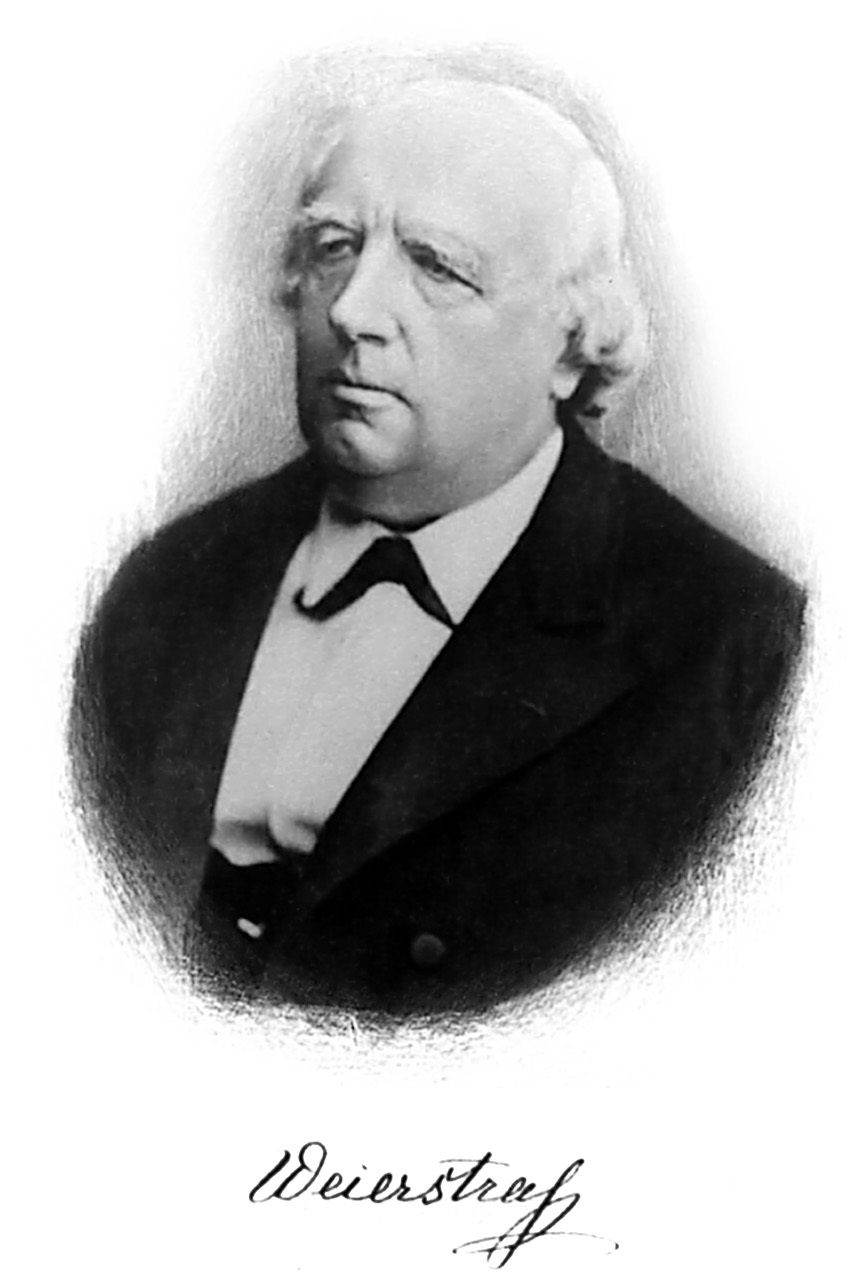
\includegraphics[width=5cm,height=6.5cm]{Karl_Weierstrass.jpg}}
    \caption{Retrato de Karl Weierstrass. Fuente: Wikimedia Commons.}
    \label{fig:weierstrass}
\end{figure}
\end{minipage}

\begin{definicion}[Límite de una función de $n$ variables]
Dada la función de $n$ variables $f:D \subseteq \mathbb{R}^m  \mapsto \mathbb{R}^n$, $f(x_1,x_2,...,x_n)$, entonces, diremos que el límite de $f$ conforme nos acercamos a la coordenada $(a_1,a_2,...,a_n)$ es igual a $L$, denotado por:
\[
\lim_{(x_1,x_2,...,x_n)\to (a_1,a_2,...,a_n)}f(x_1,x_2,...,x_n) = L
\]
Si para todo $\varepsilon>0$, existe algún $\delta>0$, tal que:
\[
0<\sqrt{(x_1-a_1)^2+(x_2-a_2)^2+...+(x_n-a_n)^2}<\delta \Rightarrow |f(x_1,x_2,...,x_n)-L|<\varepsilon
\]

\end{definicion}


\newpage
\section{Continuidad}

Cuando estudiamos la continuidad para funciones de una variable, hicimos énfasis en que la continuidad en algún punto $x=a$ es posible sólo si la función evaluada en $a$, es decir, la imagen de $a$, es el mismo valor que obtenemos al calcular el límite de esta función al hacer que $x$ tienda a $a$, esto es:
\[
\lim_{x\to a} f(x) = f(a)
\]

De cumplirse esto, podemos decir que $f(x)$ es continua en $a$. Este mismo concepto de continuidad para funciones de una variable se puede extender a funciones de $n$ variables en general.

\begin{definicion}[Continuidad de una función de $n$ variables]
Una función de varias variables $f(x_1,x_2,...,x_n)$ se dice \textbf{continua} en un punto $(a_1,a_2,...,a_n)$ si se cumple que:
\[
\lim_{(x_1,x_2,...,x_n)\to (a_1,a_2,...,a_n)}f(x_1,x_2,...,x_n) = f(a_1,a_2,...,a_n)
\]
\end{definicion}

Si la definición anterior aún le resulta algo oscura, no es necesario preocuparse (todavía...), dado que usualmente en cursos de cálculo de ingeniería, se suele comenzar estudiando casos de 2 o a lo más 3 variables.

\begin{definicion}[Continuidad de una función de $2$ variables]
Una función de varias variables $f(x,y)$ se dice \textbf{continua} en un punto $(a,b)$ si se cumple que:
\[
\lim_{(x,y)\to (a,b)}f(x,y) = f(a,b)
\]
\end{definicion}


\newpage
\section{Cálculo de límites de funciones en varias variables}

\subsection{Método de sustitución directa}

Comenzamos revisando el caso más trivial, es decir, que el problema quede resuelto inmediatamente al sustituir directamente los valores numéricos del punto en la función.

\begin{ejemplo}
Dada la función $f(x,y)=x^2+y^2$, estudiar:
\[
\lim_{(x,y)\to(1,2)}(x^2+y^2)
\]
\end{ejemplo}
\textbf{Solución:}
\begin{itemize}
    \item Como la función es continua, simplemente sustituimos:
        \[
        1^2+2^2=1+4=5
        \]
    \item Por lo tanto:
        \[
        \lim_{(x,y)\to(1,2)}(x^2+y^2)=5
        \]
\end{itemize}

\begin{ejemplo}
Dada la función $f(x,y)=e^x \cos(y)$, estudiar:
\[
\lim_{(x,y)\to(0,0)}
\]
\end{ejemplo}

\textbf{Solución:}
\begin{itemize}
    \item Como la función es continua, simplemente sustituimos:
    \[
    e^0 \cos(0) = 1 \cdot 1 = 1
    \]
    \item Por lo tanto:
    \[
    \lim_{(x,y)\to(0,0)}e^x \cos(y)=1
    \]
\end{itemize}

\newpage
\subsection{Método de aproximación por los ejes}

\begin{minipage}[t]{0.5\textwidth}
\hspace*{0.65cm}En este método utilizamos las 2 trayectorias más sencillas posibles, estas son los mismos ejes X e Y, por tanto sólo basta con hacer $x=0$ o bien $y=0$.

\hspace*{0.65cm}Este método resulta útil para verificar rápidamente casos donde el límite no existe, sin embargo no permite demostrar existencia.

\hspace*{0.65cm}Veámos a continuación dos ejemplos para comprobarlo:
\end{minipage}
\hspace{10mm} 
\begin{minipage}[t]{0.4\textwidth}
\vspace{-0.8cm}
\begin{figure}[H]
    \centering
    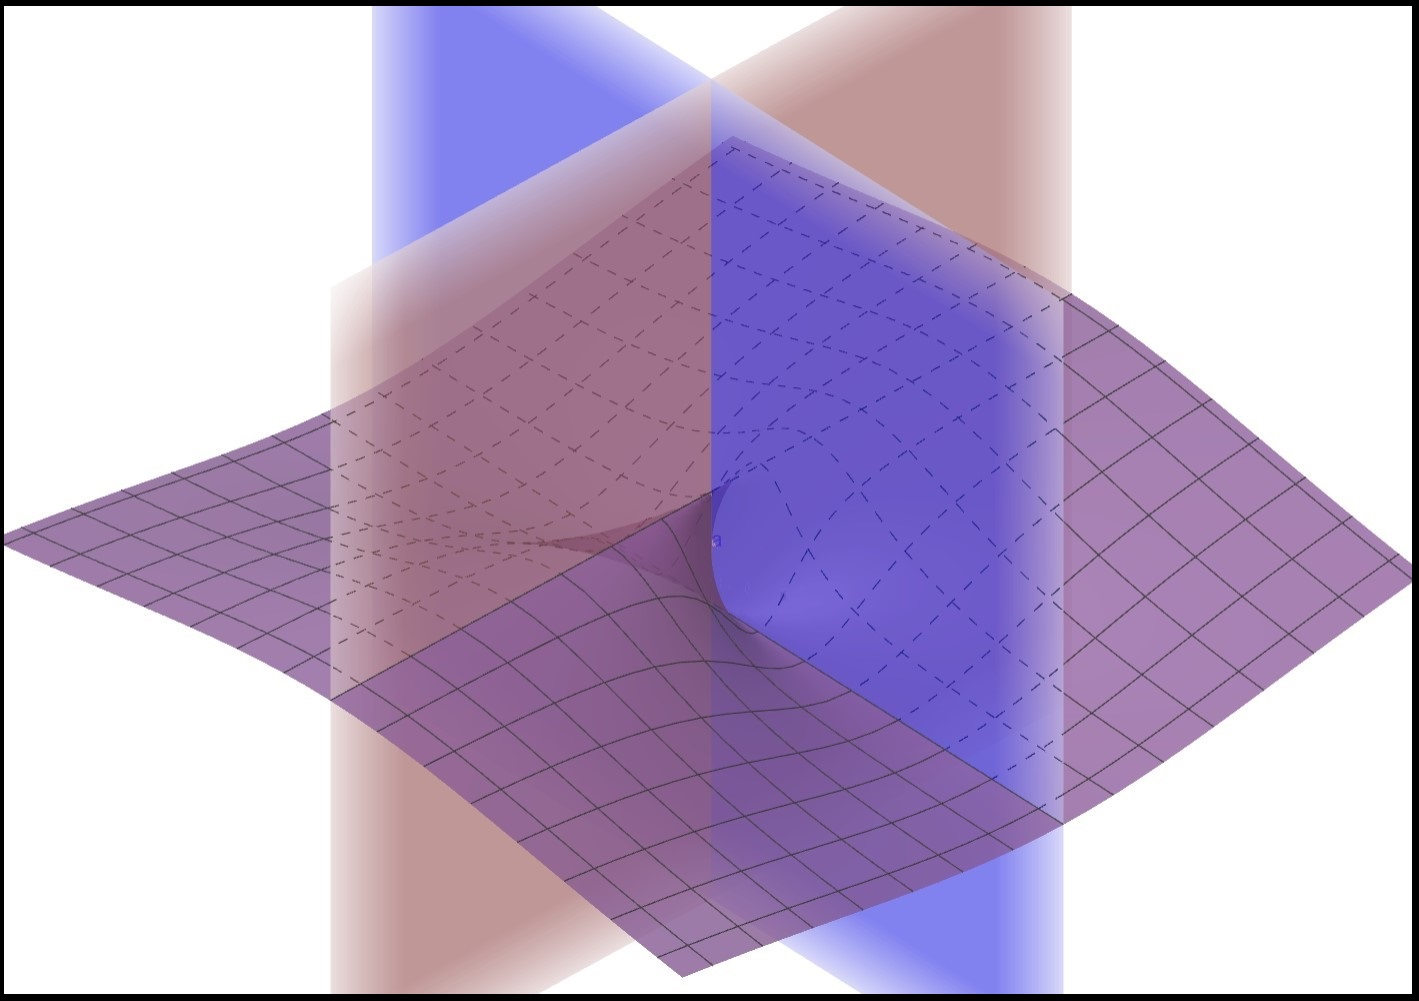
\includegraphics[width=0.9\textwidth]{C3.jpg}
    \caption{Ejemplo de aproximación por los ejes.
    En color \textcolor{blue}{azul} el plano de $x=0$ y en color \textcolor{red}{rojo} el plano de $y=0$.}
    \label{fig:aproximacion_ejes}    
\end{figure}
\end{minipage}

\begin{ejemplo}[un caso donde se demuestra no existencia]
Dada la función $f(x,y)=\dfrac{x^2-y^2}{x^2+y^2}$, estudiar:
\[
\lim_{(x,y)\to(0,0)}\dfrac{x^2-y^2}{x^2+y^2}
\]
\end{ejemplo}
\textbf{Solución:}
\begin{itemize}
    \item Primero probamos por el eje $x$ (es decir, $y=0$). Entonces:
        \[
        f(x,0)=\frac{x^2-0^2}{x^2+0^2}=\dfrac{x^2}{x^2}=1
        \]

    \item Ahora probamos por el eje $y$ (es decir, $x=0$). Entonces:
        \[
        f(0,y)=\frac{0^2-y^2}{0^2+y^2}=\dfrac{-y^2}{y^2}=-1
        \]
    \item Como los dos resultados son diferentes, el límite no existe.
\end{itemize}
\newpage
\begin{ejemplo}[un caso donde este método no demuestra]
Dada la función $f(x,y)=\dfrac{xy}{x^2+y^2}$, estudiar:
\[
\lim_{(x,y)\to(0,0)}\dfrac{xy}{x^2+y^2}
\]
\end{ejemplo}
\textbf{Solución:}
\begin{itemize}
    \item Primero probamos por el eje $x$ (es decir, $y=0$). Entonces:
        \[
        f(x,0)=\frac{x(0)}{x^2+0}=0
        \]

    \item Ahora probamos por el eje $y$ (es decir, $x=0$). Entonces:
        \[
        f(0,y)=\frac{0(y)}{0+y^2}=0
        \]
    \item Ambos caminos dan 0. Pero esto todavía \textbf{no demuestra que el límite exista}, pues podrían existir otras trayectorias por las que podríamos obtener otros valores diferentes.
\end{itemize}

\subsection{Método de rectas generales}

En el caso anterior, sólo utilizabamos 2 rectas para verificar la \textbf{no existencia} de un límite. Tendría sentido que el enfoque sea ahora generalizar este método para cualquier recta que pase por el origen, esto es, la forma $y=mx$.

Si bien, ahora podremos comprobar más eficientemente casos de \textbf{no existencia}, aún no podremos demostrar la existencia del límite, pues puede llegar a suceder, en ciertos casos, que todas las trayectorias de la forma $y=mx$ nos den el mismo resultado numérico y no obstante, existir alguna trayectoria diferente a esta que pudiese dar otro resultado distinto.

\begin{ejemplo}[caso donde este método sirve]
Dada la función $f(x,y)=\dfrac{xy}{x^2+y^2}$, estudiar:
\[
\lim_{(x,y)\to(0,0)}\dfrac{xy}{x^2+y^2}
\]
\end{ejemplo}
\textbf{Solución:}
\begin{itemize}
    \item Resulta sencillo comprobar que si aplicamos el \textbf{método de aproximación por los ejes}, el resultado no es concluyente (se propone como ejercicio al lector verificar esto).
    \item Probaremos usar \textbf{rectas generales de la forma $y=mx$}:
    \[
    f(x,mx)=\dfrac{x(mx)}{x^2+(mx)^2}=\dfrac{mx^2}{x^2(1+m^2)}=\dfrac{m}{1+m^2}
    \]
    \item Esto quiere decir que el resultado dependerá de la $m$ (la pendiente de la recta). Probaremos algunos casos particulares:
    \begin{enumerate}
        \item[-] Si $m=0 \Rightarrow \dfrac{m}{1+m^2}=0$
        \item[-] Si $m=1 \Rightarrow \dfrac{m}{1+m^2}=\dfrac{1}{2}$
    \end{enumerate}
    \item Ambos caminos dan resultados diferentes, por tanto el límite no existe.
\end{itemize}

\begin{ejemplo}[caso donde este método no sirve]
Dada la función $f(x,y)=\dfrac{x^2y}{x^4+y^2}$, estudiar:
\[
\lim_{(x,y)\to(0,0)}\dfrac{x^2y}{x^4+y^2}
\]
\end{ejemplo}
\textbf{Solución:}
\begin{itemize}
    \item Probaremos usar \textbf{rectas generales de la forma $y=mx$}:
        \begin{align*}
        \lim_{(x,y)\to(0,0)}\dfrac{x^2y}{x^4+y^2} &=\lim_{x\to 0}\dfrac{x^2(mx)}{x^4+(mx)^2} \\
        &=\lim_{x\to 0} \dfrac{mx^3}{x^4+m^2x^2}\\
        &=\lim_{x\to 0} \dfrac{mx^3}{x^2(x^2+m^2)}\\
        &=\lim_{x\to 0} \dfrac{mx}{x^2+m^2}\\
        &=\dfrac{m(0)}{(0)^2+m^2}\\
        &=0
        \end{align*}
    \item Esto quiere decir que obtenemos 0 para toda recta de la forma $y=mx$, sin embargo hay trayectoria diferentes que podrían llevarnos a otro resultado. Por lo tanto, este método no permite decidir si es que este límite existe.
\end{itemize}

\subsection{Método de curvas especiales}

El ejemplo anterior podría tener solución si intentamos aproximarnos por otra trayectoria que no sea una recta. Aquí podríamos probar con gran variedad de casos, por ejemplo:
\[
y=x^2 \qquad ; \qquad y=x^3 \qquad ; \qquad y=x^n \qquad ; \qquad y=\sqrt{x}
\]

Probaremos ahora, calcular el mismo límite del ejempo anterior pero a través de una trayectoria diferente.

\begin{ejemplo}[probando una trayectoria parabólica]
Dada la función $f(x,y)=\dfrac{x^2y}{x^4+y^2}$, estudiar:
\[
\lim_{(x,y)\to(0,0)}\dfrac{x^2y}{x^4+y^2}
\]
\end{ejemplo}
\textbf{Solución:}
\begin{itemize}
    \item Vimos en el ejemplo anterior que usando cualquier recta $y=mx$ el resltado sería siempre 0.
    \item Probaremos ahora, usar \textbf{rectas generales de la forma $y=x^2$}:
        \begin{align*}
        \lim_{(x,y)\to(0,0)}\dfrac{x^2y}{x^4+y^2} &=\lim_{x\to 0}\dfrac{x^2(x^2)}{x^4+(x^2)^2} \\
        &=\lim_{x\to 0} \dfrac{x^4}{x^4+x^4}\\
        &=\lim_{x\to 0} \dfrac{x^4}{2x^4}\\
        &=\lim_{x\to 0} \dfrac{1}{2}\\
        &=\dfrac{1}{2}
        \end{align*}
    \item Entonces, ciertas trayectorias dan 0, pero otras dan $\tfrac{1}{2}$. Por lo tanto, acabamos de comprobar que este límite no existe.
\end{itemize}

% \subsection{Comparación de órdenes de magnitud}
% Ejemplo:
% \[
% f(x,y)=\frac{x^3y}{x^6+y^2}
% \]
% Queremos encontrar una curva que haga competir ambos términos del denominador:
% \[
% x^6\sim y^2
% \]
% Entonces:
% \[
% y=x^3
% \]
% Sustituyendo:
% \[
% f(x,x^3)=\frac{x^3(x^3)}{x^6+x^6}
% \]
% \[
% =\frac{x^6}{2x^6}
% \]
% \[
% =\frac12
% \]
% Mientras que por $y=0$:
% \[
% f(x,0)=0
% \]
% Entonces el límite no existe.

\subsection{Método de coordenadas polares}

Cuando trabajamos con curvas planas, cuya representación geométrica es simétrica respecto de un punto, podemos usar coordenadas polares para obtener expresiones algebraicas mucho más simples. Recordemos que la transformación a coordenadas polares está caracterizada por:
\[
x =r \cos (\theta) \qquad ; \qquad y =r \sin (\theta) \qquad ; \qquad x^2 + y^2 = r^2
\]

En varias variables, no siempre tendremos claridad de la representación geométrica de la funciones, salvo ciertas superficies conocidas. No obstante, podemos inferir que resultará conveniente aplicar coordenadas polares cuando la función presente términos de la forma:
\[
x^2 + y^2 \qquad \text{, o bien:} \qquad \sqrt{x^2 + y^2}
\]


\begin{ejemplo}
Dada la función
\[
f(x,y)=\frac{x^2y^2}{x^2+y^2}
\]
Queremos estudiar:
\[
\lim_{(x,y)\to(0,0)}\frac{x^2y^2}{x^2+y^2}
\] 
\end{ejemplo}
\textbf{Solución:}
\begin{itemize}
    \item Tanto si usamos método de \textbf{aproximación por los ejes}, como el de \textbf{rectas generales}, obtenemos siempre 0 como resultado (verificarlo).
    \item Dado que la función presenta un término de la forma $x^2+yu^2$, probaremos cambiar a coordenadas polares:
        \begin{align*}
        \lim_{(x,y)\to(0,0)}\frac{x^2y^2}{x^2+y^2} &=\lim_{r \to 0}\dfrac{(r \cos (\theta))^2(r \sin (\theta))^2}{r^2} \\
        &=\lim_{r \to 0}\dfrac{r^2 \cos^2 (\theta) r^2 \sin^2 (\theta)}{r^2} \\
        &=\lim_{r \to 0} r^2 \cos^2 (\theta)  \sin^2 (\theta)
        \end{align*}
    \item En este punto, dado que $r^2$ tiende a cero y el factor angular $\cos^2 (\theta)  \sin^2 (\theta)$ está acotado (para cualquier $\theta$, sólo varía entre 0 y 1), podemos concluir que el límite existe y es 0.
\end{itemize}

\begin{nota}
Pese a que escribimos $r \to 0$, siempre debemos revisar que la solución sea uniformemente válida para cualquier $\theta$. Por ejemplo, si obtenemos una expresión como:
\[
\lim_{r\to 0}\frac{r}{\sin \theta}
\] 
no podríamos concluir nada sólo con $r \to 0$, pues la expresión $1/\sin \theta$ no está acotada.
\end{nota}

% \subsection{Dependencia de $\theta$ en polares}
% Ejemplo:
% \[
% f(x,y)=\frac{x^2}{x^2+y^2}
% \]
% Usando polares:
% \[
% \frac{r^2\cos^2\theta}{r^2}
% \]
% \[
% =\cos^2\theta
% \]
% El resultado depende de $\theta$.Por ejemplo:
% \begin{itemize}
%     \item Si $\theta=0$:
%     \[
%     1
%     \]

%     \item Si $\theta=\frac{\pi}{2}$:
%     \[
%     0
%     \]
% \end{itemize}
% Entonces el límite no existe.

% \subsection{Acotación}
% Ejemplo:
% \[
% f(x,y)=\frac{x^2y^2}{x^2+y^2}
% \]
% Sabemos que:
% \[
% x^2y^2\le (x^2+y^2)^2
% \]
% Entonces:
% \[
% 0\le \frac{x^2y^2}{x^2+y^2}\le x^2+y^2
% \]
% Y como:
% \[
% x^2+y^2\to 0
% \]
% por el teorema del sandwich:
% \[
% \frac{x^2y^2}{x^2+y^2}\to 0
% \]

% \subsection{Método de curvas paramétricas específicas}
% Ejemplo:
% \[
% f(x,y)=\frac{x^2y}{x^4+y^2}
% \]
% Tomamos:
% \[
% x=t
% \]
% \[
% y=t^2
% \]
% Entonces:
% \[
% f(t,t^2)=\frac{t^2(t^2)}{t^4+t^4}
% \]
% \[
% =\frac{t^4}{2t^4}
% \]
% \[
% =\frac12
% \]

\newpage
\subsection{Método de curvas paramétricas generalizadas}

Si ya hemos agotado los métodos anteriores y aún no podemos concluir sobre la existencia o no existencia de un límite en varias variables, podemos recurrir al método de \textbf{curvas para métricas generalizadas}.
\vspace{0.5cm}

{\Large\textbf{Resumen del método:}}
\begin{enumerate}[label=\roman*.]
    \item Aplicaremos el método cuando $(x,y)$ tienda a $(0,0)$. Si tiende a cualquier otro punto $(a,b)$ podemos aplicar primero traslación de ejes $u=x-a$ y $v=y-b$.
    \item Identificar si existen expresiones de la forma: $x^a \pm y^b$, tales como:
\[
x-y \qquad ; \qquad x-y^2 \qquad ; \qquad x^2 + y^4
\]
    \item Aplicamos una parametrización de la forma:
    $$\begin{cases} x = t \\ y = t \cdot h(t) \end{cases}$$
    ¿Por qué? porque así aseguramos que la curva pase por el origen, pues $\lim_{t \to 0} t \cdot h(t)=0$
    \item Sustituimos en la función y analizamos el resultado en función de lo que valga el límite de $h(t)$ cuando $t \to 0$.
    \item Si al final el resultado del límite depende de la forma de $h(t)$, entonces el límite no existe, porque diferentes funciones $h(t)$ (diferentes trayectorias) dan resultados distintos.
\end{enumerate}

\begin{ejemplo}
    Estudiar:
    \[
    \lim_{(x,y) \to (0,0)}\frac{x^2y^2}{x^2y^2+(x-y)^2}
    \]
\end{ejemplo}
\textbf{Solución:}
\begin{itemize}
    \item Observamos que hay presencia del término $(x-y)^2$.
    \item Aplicamos la parametrización de curva general:
    $$\begin{cases} x = t \\ y = t \cdot h(t) \end{cases}$$
    \item Sustituyendo, factorizando y simplificando:
    \begin{align}
        \lim_{(x,y) \to (0,0)}\frac{x^2y^2}{x^2y^2+(x-y)^2} &= \lim_{t \to 0}\frac{t^2[th(t)]^2}{t^2[th(t)]^2+[t-th(t)]^2} \\
         &= \lim_{t \to 0}\frac{t^2h(t)^2}{t^2h(t)^2+[1-h(t)]^2} 
        \label{limite_parametrico_generalizado_1}
    \end{align}
    \item Este resultado claramente depende del $h(t)$ que se escoja, pero para probar que el límite no existe debemos encontrar un par de casos con resultados diferentes. Por ejemplo:
    \begin{enumerate}
        \item[-] Si $h(t) \to 0$, entonces el límite es cero.
        \begin{align*}
        \lim_{h(t) \to 0}\frac{t^2h(t)^2}{t^2h(t)^2+[1-h(t)]^2} 
         &= \lim_{t \to 0}\frac{t^2(0)^2}{t^2(0)^2+[1-(0)]^2}=\dfrac{0}{1}=0
        \end{align*}
        \item[-] Si $h(t) \to \infty$, entonces el límite es cero.
        \begin{align*}
        \lim_{h \to \infty}\frac{t^2h^2}{t^2h^2+[1-h]^2} 
         &= \lim_{h \to \infty}\frac{t^2h^2}{t^2h^2+1-2h+h^2}\\
         &= \lim_{h \to \infty}\frac{t^2h^2}{(t^2+1)h^2+1-2h} \cdot \dfrac{1/h^2}{1/h^2}\\
         &= \lim_{h \to \infty}\frac{t^2}{(t^2+1)+1/h^2-2/h}\\
         &= \frac{t^2}{(t^2+1)}
        \end{align*}
        desde aquí resulta claro que si $t \to 0$ entonces resulta cero.
        \item[-] Si $h(t) \to k \neq 0$, se obtendrá también cero, excepto cuando $k=1$.
        \begin{align*}
        \lim_{t \to 0} \left( \lim_{h \to k}\frac{t^2h^2}{t^2h^2+[1-h]^2} \right) 
         &= \lim_{t \to 0}  \frac{t^2k^2}{t^2k^2+[1-k]^2}=\dfrac{0}{(1-k)^2} 
        \end{align*}
    \end{enumerate}
    \item El análisis anterior nos deja la interrogante de qué sucede cuando:
    \[
    \lim_{t \to 0} h(t) = 1
    \]
    Para ello, escogemos un $h(t)$ cuyo límite sea 1 cuando $t$ tienda a cero, y la opción más simple puede ser $h(t)=1-t$, pues:
    \[
    \lim_{t \to 0} (1-t) = 1
    \]
    \item Sustituyendo $h(t)=1-t$ en (\ref{limite_parametrico_generalizado_1}):
    \begin{align*}
        \lim_{t \to 0}\frac{t^2h^2}{t^2h^2+[1-h]^2} 
         &= \lim_{t \to 0}\frac{t^2(1-t)^2}{t^2(1-t)^2+[1-(1-t)]^2}\\
         &= \lim_{t \to 0}\frac{t^2(1-t)^2}{t^2(1-t)^2+t^2}\\
         &= \lim_{t \to 0}\frac{(1-t)^2}{(1-t)^2+1}\\
         &= \frac{(1-0)^2}{(1-0)^2+1}\\
         &= \dfrac{1}{2}\neq 0
    \end{align*}
    \item Por lo tanto, hemos encontrado trayectorias que dan como resultado cero y otras que dan como resultado $1/2$, por lo tanto, el límite no existe.
\end{itemize}


% \subsection{Cambio de variables especial}
% Ejemplo:
% \[
% f(x,y)=\frac{x+y}{x-y}
% \]
% Aquí aparece repetidamente:
% \[
% x-y
% \]
% Entonces conviene definir:
% \[
% u=x-y
% \]
% \[
% v=x+y
% \]
% La función queda:
% \[
% \frac{v}{u}
% \]
% Esto puede simplificar mucho algunos problemas avanzados.
